\section{Interfejs NFC}
\label{NFC}

Poniższy rozdział powstał na podstawie źródeł \cite{NFC} i \cite{NFC_NXP}.\\

Near Field Communication to protokół radiowy, stanowiący rozszerzenie swego starszego brata - interfejsu RFID. Mimo, iż jest do niego bardzo podobny w wielu aspektach, różni się znacznie pod względem założeń. RFID (\textit{ang. \textbf{R}adio \textbf{F}requency \textbf{Id}entification}), nie stanowi prawdziwego protokołu komunikacyjnego, bowiem pozwala jedynię na wymianę bardzo krótkich informacji, zwanych identyfikatorami. Urządzenia RFID stanowią bardzo proste układy. Składają się one zazwyczaj z niewielkiego chipa, zawierającego pamięć nieulotną (zazwyczaj do 1 kB) oraz anteny. Przedstawiono to na rysunku \ref{fig:image_rfid_tag}.

\begin{figure}[H]
	\centering
	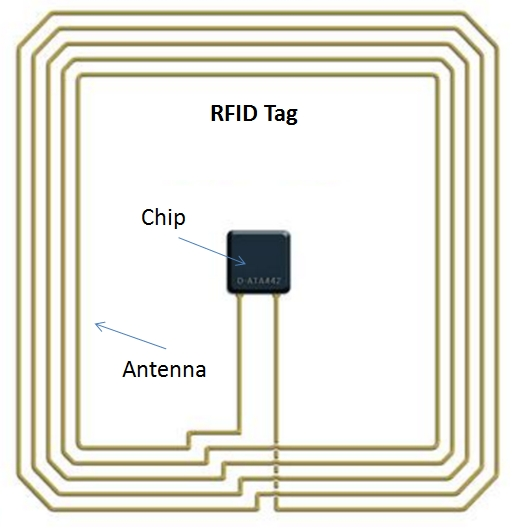
\includegraphics[width=10cm]{img/theory/NFC/RFID_tag.jpg}
	\caption{Budowa tag'a RFID. Źródło: \cite{RFID_antenna}}
	\label{fig:image_rfid_tag}
\end{figure}

W odróżnieniu od tego, NFC (\textit{ang. \textbf{N}ear \textbf{F}ield \textbf{C}ommunication}) stanowi pełnoprawny protokół komunikacyjny. Umożliwia on wymianę długich wiadomości. Został on zbudowany na podstawie RFID i wykorzystuje jego warstwę fizyczną. Tak samo jak w RFID, w NFC można wyróżnić 2 typy urządzeń - pasywne oraz aktywne. Urządzenie pasywne nie generuje swojego własnego pola elektromagnetycznego, w przeciwieństwie do do urządzenia aktywnego, które inicjuje komunikację. Ponadto, urządzenie bierne, tak samo jak w przypadku RFID nie posiada nawet własnego źródła zasilania. Gdy znajdzie się ono w polu wygenerowanym przez urządzenie aktywne, w jego antenie wyindukuje się prąd, który jest w stanie zasilić niewielki moduł. Komunikacja zwrotna odbywa się poprzez modyfikację zużycia energii tag'a (urządzenia pasywnego) zgodnie z bitowym wzorcem, który należy wysłać. Dynamiczne zmiany parametrów zużycia powodują pewne zaburzenia wygenerowanego przez inicjator pola RF. Odczyt danych przez nie polega na odczycie zmian tego pola. Przedstawiono to na rysunku \ref{fig:image_nfc_comm}. 

\begin{figure}[H]
	\centering
	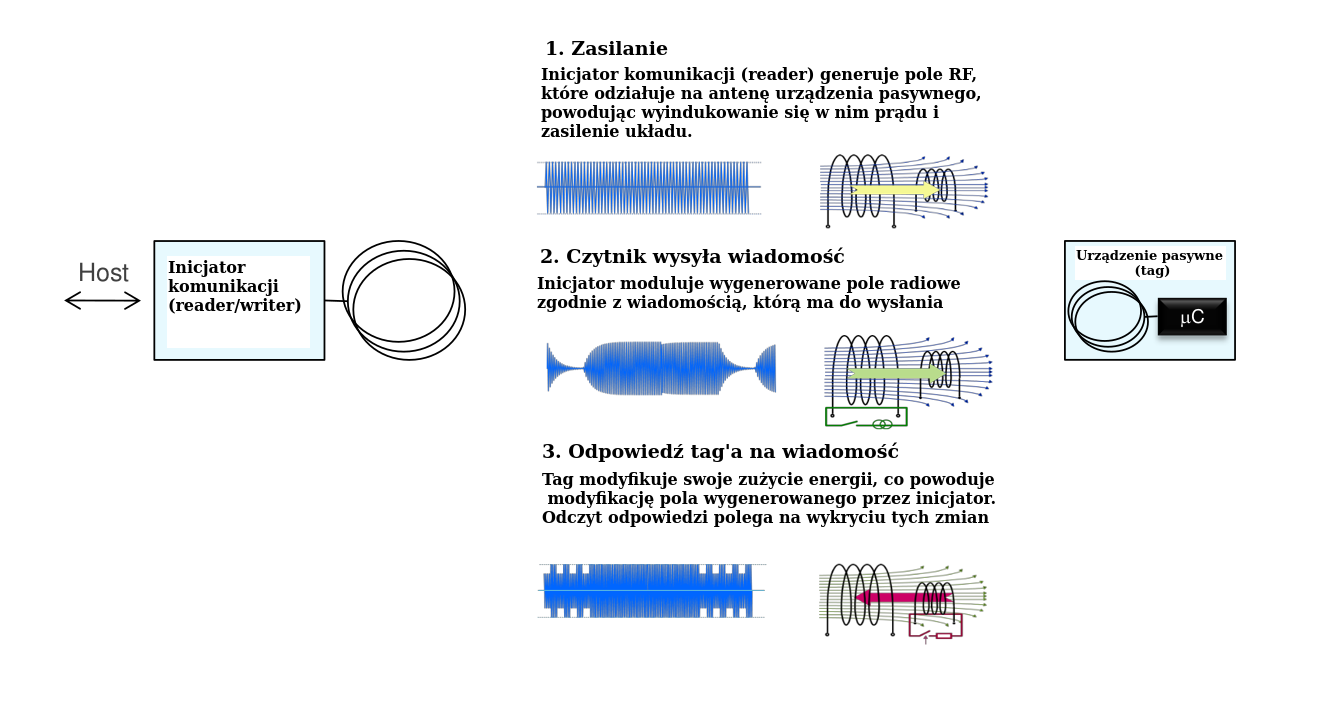
\includegraphics[width=18cm]{img/theory/NFC/NFC_communication.png}
	\caption{Zasada działania komunikacji pomiędzy urządzeniem aktywnym i pasywnym. Źródło: \cite{NFC_NXP}}
	\label{fig:image_nfc_comm}
\end{figure}

Istnieje również możliwość komunikacji pomiędzy dwoma urządzeniami aktywnymi, wówczas zamiast modyfikować pole wyindukowane, urządzenie odpowiada swoim własnym, wygenerowanym z energii źródła zasilania polem. Dzięki temu zasięg komunikacji jest większy. 

Na tym w zasadzie podobieństwa między NFC i RFID się kończą. RFID pozwala bowiem na odpowiedź w postaci swojegu unikalnego numeru identyfikacyjnego UID (\textit{ang. \textbf{U}nique \textbf{I}dentifier \textbf{N}umber}, natomiast moduły NFC stanowią najczęściej urządzenia programowalne, co pozwala na przesłanie dowolnej wiadomości. Ponadto, kolejną różnicą jest fakt, że nie posiada jednego wspólnego standardu komunikacji. Co więcej, nie posiada nawet stałej częstotliwości komunikacji, lecz zależy ona od producenta sprzętu.  Zasięg komunikacji w przypadku RFID również jest zmienny i zależny od częstotliwości sygnału. Dla wartości rzędu 125 - 134.3 kHz wynosi ona do 30 cm (zazwyczaj około 10 cm), dla częstotliwości 13.56 MHz - do 1.5 metra, a w przypadku 433 MHz - nawet do 500 metrów. Ta różnorodność i brak pojedynczego standardu komunikacji stała się przyczyną do powstania protokołu NFC.

NFC pracuje na pojedynczej częstotliwości o wartości 13.56 MHz. Zasięg komunikacji jest niewielki (rzędu 10 cm). Ponadto mają możliwość emulowania tagów RFID, czyli zachowania się jak one gdy wykryte zostanie pole RF. Dodatkowym atutem NFC jest zdefiniowanie formatu komunikacji pomiędzy urządzeniami - NDEF (\textit{ang. \textbf{N}FC \textbf{D}ata \textbf{E}xchange \textbf{F}ormat}). Istnieją pewne dobrze znane struktury danych, możliwe do wysłania poprzez NFC. Są to:

\begin{itemize}
\item Wiadomości tekstowe
\item Adresy internetowe URI
\item Proste komendy
\item Podpisy cyfrowe
\end{itemize}

Organizacją zajmującą się standaryzacją i rozwijaniem NFC jest NFC Forum. Definiuje ono 4 rodzaje urządzeń pasywnych:

\begin{enumerate}
	\item Typ 1
	\begin{itemize}
		\item Bazuje na specyfikacji ISO-14443A
		\item Może być tylko do odczytu lub mieć zdolność do zapisu i odczytu
		\item Rozmiar pamięci od 96 B do 2 kB
		\item Prędkość komunikacji - 106 kb/s
		\item Brak ochrony przed kolizją pól
	\end{itemize}
	
	\item Typ 2
	\begin{itemize}
		\item Bazuje na specyfikacji ISO-14443A
		\item Może być tylko do odczytu lub mieć zdolność do zapisu i odczytu
		\item Rozmiar pamięci od 96 B do 2 kB
		\item Prędkość komunikacji - 106 kb/s
		\item Zapewnia mechanizm ochrony przed kolizją
	\end{itemize}
	
	\item Typ 3
	\begin{itemize}
		\item Bazuje na specyfikacji ISO-18092 i JS-X-6319-4
		\item Może być tylko do odczytu lub mieć zdolność do zapisu i odczytu
		\item Rozmiar pamięci do 1 MB
		\item Prędkość komunikacji - 212 lub 424 kb/s
		\item Zapewnia mechanizm ochrony przed kolizją
	\end{itemize}
	
	\item Typ 4
	\begin{itemize}
		\item Bazuje na specyfikacji ISO-18092 i JS-X-6319-4
		\item Może być tylko do odczytu lub mieć zdolność do zapisu i odczytu
		\item Rozmiar pamięci: 2, 4 lub 8 kB
		\item Prędkość komunikacji - 106, 212 lub 424 kb/s
		\item Zapewnia mechanizm ochrony przed kolizją
	\end{itemize}
	
\end{enumerate}


